\section{Design}
\label{sec:Design}

\subsection{Architecture Design}
\label{sec:Design>Architecture Design}
Because we selected the web application model from the beginning, the classic client-server web architecture was quickly adopted. The architecture is a distributed application structure that partitions tasks or workloads between the providers of a resource or service, called servers, and service requests called clients. In theory, any device connected to the Internet can try to access and obtain the resources or services of the server while the server is running normally. Based on the client-server structure, we have detailed its component structures below \cite{web:Architecture-design}:

\subsubsection{Web Browser or Client}
\label{sec:Design>Architecture Design>Web Browser or Client}
The web browser or client is the interface rendition of a web app functionality, with which the user interacts. This content delivered to the client is developed using HTML, JavaScript, and CSS and does not require operating system related adaptations. In essence, the web browser or client manages how end users interact with the application.

There are three, well-known Web Application Architecture types available in the modern landscape: Single Page Applications (SPA), Microservices, and Serverless Architectures. Because SPA provides more responsive user experience and clean separation between data and views. Furthermore, our frontend and backend are developed separately. We chose the SPA structure.

The SPA model interacts with the user by providing updated content within the current page rather than loading entirely new pages from the server with each action from the user. It helps prevent interruptions in the user experience, transforming the behavior of the application such that it resembles a traditional desktop application.

\subsubsection{Web Application Server}
\label{sec:Design>Architecture Design>Web Application Server}
The web application server manages business logic and data persistence and can be built using PHP, Python, Java, Ruby, .NET, Node.js, among other languages. It is comprised of at least a centralized hub or control center to support multi-layer applications. The essential purpose of a web server architecture is to complete requests made by clients for a website. The clients are typically browsers and mobile apps that make requests using secure HTTPs protocol, either for page resources or a REST API.

Since the focus of this project is on the client side (frontend), which is the map generator (written in JavaScript), we chose Node.js. Moreover, Node.js is written using JavaScript and is the same technology as the frontend components. This makes it easier for the developer to program backend services and frontend user interfaces simultaneously. It also provides consistency, code sharing and reusability, simple knowledge-transfer, and a large number of free tools. These benefits bring flexibility and efficiency when building this project.

\subsubsection{Database Server}
\label{sec:Design>Architecture Design>Database Server}
The database server provides and stores relevant data for the application. Additionally, it may also supply the business logic and other information that is managed by the web application server. There are multiple popular database systems available: Oracle, MySQL, Microsoft SQL Server, PostgreSQL, MongoDB, MariaDB, DB2, and SAP HANA.

Because the project involves a small number of entities, the relationships among entities are not complicated, and the choice of the Software Development Life Cycle (SDLC) model, we chose MongoDB, which is dynamic, flexible and easy to get started. It also provides high performance, high availability, and high scalability. More importantly, our main purpose is to save maps and implement basic CRUD (create, retrieve, update, delete) operations of the database. As MongoDB is a schema-less database (written in C++), we can serialize the map data to JSON, send it to MongoDB and then save it.

\subsection{Database Design}
\label{sec:Design>Database Design}
NoSQL stands for ``Not only SQL," which is an approach to database design that can accommodate a wide variety of data models, including key-value, document, columnar and graph formats. MongoDB is a type of NoSQL database. A record in MongoDB is a document, which is a data structure composed of field and value pairs. MongoDB documents are similar to JSON objects, because the values of fields may include other documents, arrays, and arrays of documents.

The system supports only two document types: the user and the map. A user can have many maps, but a map can only belong to one user. Thus, the relationship between the user and the map should be one-to-many.

MongoDB provides two ways of data modeling: Embedded Data Modeling and Normalized Data Modeling. Using Embedded Data Modeling, we may embed related data in a single structure or document, which means we should store maps in the user schema. However, the data of the map is relatively large, in general, it may exceed the maximum BSON document size set by MongoDB, and the map cannot exist as a separate entity. Though embedding provides better performance for reading operations, as well as the ability to request and retrieve related data in a single database operation, it is still beyond our consideration.

Normalized Data Modeling provides One-to-One and One-to-Many Relationships. We chose the Normalized One-to-Many Structure, which uses references between documents, and provides more flexibility than embedding. Figure \ref{fig:ER Diagram} is the Entity Relationship Diagram that describes the relationship between the user and the map.

\begin{figure}[htbp]
\centering
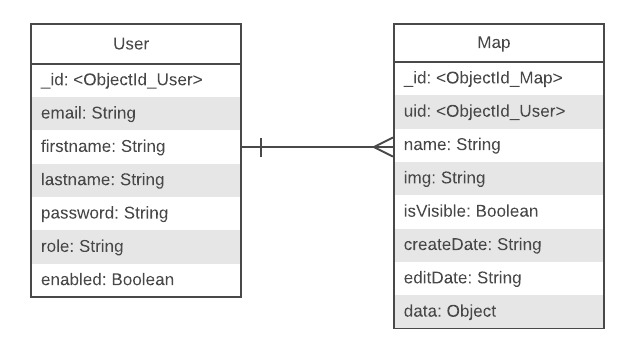
\includegraphics[width=\textwidth]{section03/assets/ER_Diagram.png}
\caption[Entity Relationship Diagram]{\label{fig:ER Diagram}Entity Relationship Diagram}
\end{figure}

\subsection{REST API Design}
\label{sec:Design>REST API Design}
An API is an application programming interface. It is a set of rules that allow programs to talk to each other. The developer creates the API on the server and allows the client to talk to it.

REST determines how the API looks like, which is the acronym for ``Representational State Transfer.'' It is an architectural style for distributed hypermedia systems and was first presented by Roy Fielding in 2000 in his famous dissertation \cite{paper:Fielding00architecturalstyles}. Like any other architectural styles, REST has its own 6 guiding constraints, which should be satisfied if an interface conforms to the RESTful. These principles are listed below:

\begin{enumerate}
  \item Client-server. By separating the user interface concerns from the data storage concerns, it improves the portability of the user interface across multiple platforms and improve scalability by simplifying the server components.
  \item Stateless. Each request from a client to server must contain all of the information necessary to understand the request, and cannot take advantage of any stored context on the server. Session state is therefore kept entirely on the client.
  \item Cacheable. Cache constraints require that the data within a response to a request be implicitly or explicitly labeled as cacheable or non-cacheable. If a response is cacheable, then a client cache is given the right to reuse that response data for later, equivalent requests.
  \item Uniform interface. By applying the software engineering principle of generality to the component interface, the overall system architecture is simplified, and the visibility of interactions is improved.
  \item Layered system. The layered system style allows an architecture to be composed of hierarchical layers by constraining component behavior such that each component cannot ``see'' beyond the immediate layer with which they are interacting.
  \item Code on demand (optional). REST allows client functionality to be extended by downloading and executing code in the form of applets or scripts. e.g., clients may call the API to get a UI widget rendering code, which is allowed.
\end{enumerate}

We found ourselves did not implement some of them, such as the Cacheable, Layered system, and Code on demand. But we were still making a RESTful API, although not “truly RESTful \cite{web:RESTArchitecturalConstraints}.” We hope to achieve them all in our future work. However, our APIs as shown in Table \ref{tab:REST API Design Table}, also implemented the rest of these principles:

\begin{enumerate}
  \item All endpoints follow a canonical form using a sequent of nested collection/item types. This practice conforms with the provision of a Uniform interface.
  \item GET requests do not alter the state, which also conforms with the provision of a Uniform interface.
  \item The client application and server application are able to evolve separately without any dependency on each other. And the client only knows resource URIs, which conforms with the provision of a Client–server.
  \item The server will not store anything about the latest HTTP request client made. It will treat each and every request as new. No session, no history. This practice conforms with the provision of a Stateless.
\end{enumerate}

\begin{table}[!htb]
  \centering
  \begin{tabularx}{\textwidth}{>{\raggedright}cXX}
    \toprule[1.5pt]
    \textbf{HTTP Verb} & \textbf{URI} & \textbf{Description}
    \\ \midrule[1.5pt]
    GET & /metro/api/v1/users & Get a list of all users
    \\ \midrule
    GET & /metro/api/v1/users/\{uid\} & Get the user with \{uid\}
    \\ \midrule
    GET & /metro/api/v1/users/\{uid\}/ maps & Get a list of all maps of the user with \{uid\}
    \\ \midrule
    PATCH & /metro/api/v1/users/\{uid\}/ password & Verify the password of the user with \{uid\}
    \\ \midrule
    PUT & /metro/api/v1/users/\{uid\}/ password & Update the password of the user with \{uid\}
    \\ \midrule
    PUT & /metro/api/v1/users/\{uid\}/ email & Update the email of the user with \{uid\} \\ \midrule
    PUT & /metro/api/v1/users/\{uid\}/ name & Update the name of the user with \{uid\} \\ \midrule
    PUT & /metro/api/v1/users/\{uid\}/ enabled & Update the enabled of the user with \{uid\}
    \\ \midrule
    GET & /metro/api/v1/maps/\{mid\} & Get the map with \{mid\}
    \\ \midrule
    GET & /metro/api/v1/maps/ ?page=\{page\}\&limit=\{limit\} & Get a list of \{limit\} maps on page \{page\}
    \\ \midrule
    POST & /metro/api/v1/maps & Add a new map to the database
    \\ \midrule
    PUT & /metro/api/v1/maps/\{mid\} & Update the map with \{mid\}
    \\ \midrule
    DELETE & /metro/api/v1/maps/\{mid\} & Delete the map with \{mid\}
    \\ \bottomrule[1.5pt]
  \end{tabularx}
  \caption[REST API Design Table]{REST API Design Table}
  \label{tab:REST API Design Table}
\end{table}

\subsection{Map Generator Design}
\label{sec:Design>Map Generator Design}
\subsubsection{Canvas and SVG}
\label{sec:Design>Map Generator Design>Canvas and SVG}
Since the project is a web application, the map generator must be able to run in the web page. We need to choose a 2D HTML graphics tool to render the map. Two technologies are available: SVG and Canvas.

SVG is a language for describing 2D graphics in XML, which means every element is available within the SVG DOM, you can attach JavaScript event handlers for an element. In SVG, each drawn shape is remembered as an object. If attributes of an SVG object are changed, the browser can automatically redraw the shape. Canvas draws 2D graphics, on the fly (with JavaScript) by rendering pixel by pixel. In Canvas, once the graphics are drawn, it is forgotten by the browser. If its position should be changed, the entire scene needs to be redrawn, including any objects that might have been covered by the graphics.

Because the map generator allows the user to annotate and edit the map, every time the user edits the map, the map will be redrawn, which contains thousands of objects, so we chose Canvas. By the way, SVG renders slowly if there are plenty of complex objects (anything that uses the DOM a lot will be slow).

\subsubsection{Graphics Libraries}
\label{sec:Design>Map Generator Design>Graphics Libraries}
There are many open source third-party graphics libraries on the web, such as D3.js, Paper.js, Fabric.js, Three.js, and so on, which provide many ready-made and mature geometric construction methods. D3.js was chosen because of the following reasons:
\begin{enumerate}
  \item It is open source: so we can freely use the library, code and build our own maps.
  \item It has good and neat documentation of all the available functions and methods.
  \item There is a gallery with unique charts that can be referred to while developing our project.
\end{enumerate}

\subsubsection{Map}
\label{sec:Design>Map Generator Design>Map}
Before we started to develop the map generator, we needed to understand what is a map and then decide what data structures and methods we are going to use to write. A map is a two-dimensional, abstract representation of the surface of the world. There are three main ways to generate a map: noise functions, random partitioning, or a hybrid of the two. Most procedural map generators use noise functions (midpoint displacement, fractal, diamond-square, Perlin noise, etc.) to generate a randomized map, but the results often look evenly artificial. So we decided to use random partitioning to model the mapping constraints. And we defined the following layers of the map:

\begin{enumerate}
  \item elevation: the elevation layer represents the altitude of the area. The elevation of all locations in a polygon is considered the same.
  \item affluence: the affluence layer represents the wealth of the district (polygon). The lower the value, the poorer the area, vice versa. It is usually used to classify residential areas.
  \item desirability: the desirability layer represents the attraction of the region to people, from 0 to infinity, which determined by elevation and affluence. People generally prefer to live in places with higher desirability.
  \item district: the district layer allows the user to assign types to districts. Correspondingly, different types of districts have different background colors. As a fantasy map of the medieval city, the city wall is always an essential element. Our map generator allows the user to create walls manually, so the user can use the warp tool to render the city wall under this layer.
  \item building: the building layer displays buildings of various districts. These buildings are procedurally generated, so the user can change them by changing the type of the district.
\end{enumerate}

Based on these layers, we have expanded the districts. A city is always composed of different regions, so we introduced the concept of type:

\begin{enumerate}
  \item rich: represents the rich area, the value of desirability is generally high
  \item medium: represents the middle-class area, the value of desirability is generally medium
  \item poor: represents slums, the value of desirability is generally low.
  \item university: represents universities and always appearing in the middle-class areas and the rich areas.
  \item park: represents parks and generally appearing at the junction of rich areas,  slums, and middle-class areas.
  \item plaza: represents plazas and generally appearing at the junction of rich areas,  slums, and middle-class areas.
  \item water: represents rivers, lakes, sea, or ocean.
  \item harbor: represents harbors, and there is usually a deck near the sea.
  \item farm: represents farms and usually there is a farmer’s house on a large farm.
  \item empty: represents empty areas.
  \item castle: represents a castle. A city map has only one castle, and the castle is always surrounded by large militaries.
  \item military: represents the military. The military always surrounds the castle
  \item religious: represents the area with churches or temples.
\end{enumerate}

After introducing these types, we want this project to have the following main features:

\begin{enumerate}
  \item Once opening the map editor page, it will show an empty map with random district placements and shapes, then the user can start editing the map.
  \item Create a map by entering the resolution of the map in the menu.
  \item View the different layers of the map, these layers can be superimposed on each other.
  \item Edit the different layers of the map.
  \item Toggle the display of street names.
  \item Set the waterline or elevation level
  \item Display contour lines or not.
  \item After selecting one or more than one layer under ``edit'' mode, the user can change the size of the "warp tool" by using the mouse wheel, which determines the area where the map will be edited.
  \item Edit the map by clicking and dragging the ``warp tool.''
  \item The districts and buildings are procedurally generated.
  \item Allow to change the type of the current district by right-clicking and selecting a new type from the context menu.
  \item Zoom in and zoom out the map by pressing on the alt key and using the mouse wheel.
  \item Use a specialized button to resize the map on the menu.
  \item Save the map.
  \item Download the map.
\end{enumerate}
